\documentclass[titlepage]{article}
\usepackage[utf8]{inputenc}
\usepackage[T1]{fontenc}
\usepackage[colorlinks=false]{hyperref}
\usepackage[a4paper]{geometry}
\usepackage{graphicx}
\usepackage{listings}
\usepackage{xcolor}
\usepackage{hyperref}
\usepackage{amsmath}

% - header and footer
\usepackage{fancyhdr}  % To customize headers and footers
\usepackage{lastpage}  % To reference the last page

\pagestyle{fancy}  % Default page style with no header
\fancyhf{}  % Clear all header/footer fields
\fancyfoot[C]{\thepage/\pageref{LastPage}}  % Page numbering in the center of the footerx

\renewcommand{\headrulewidth}{0pt}  % Remove the horizontal line under the header
\renewcommand{\footrulewidth}{0pt}  % Optional: Remove the line under the footer (if you don't want it
% ---

% - make paragraph titles look like subsubsection titles -
\usepackage{titlesec}

\titleformat{\paragraph}
{\normalfont\normalsize\bfseries}
{\theparagraph}{1em}{}

\titlespacing*{\paragraph}
{0pt}{3.25ex plus 1ex minus .2ex}{1.5ex plus .2ex}
% ---

\title{Operations Research Project}
\author{Daniel \sc Carriba Nosrati}
\date{Semestre 2 2025/2026}

\renewcommand{\contentsname}{Sommaire}

\hyphenpenalty=10000
\exhyphenpenalty=10000


\begin{document}


\begin{titlepage}
    \centering
    {\huge \bfseries Operations Research\\ Project \par}
    \vspace{1cm}
    {\Large Calculs de\\ flots maximum \& coupes minimum,\\ flots à coût minimum\\ et\\ détection de cycles à coûts négatifs\\ sur les réseaux de flot\par}
    \vfill
    {
\includegraphics[width=0.3\textwidth]{img/unice.png} \par}
    \vfill
    {\Large Daniel \sc Carriba Nosrati \par}
    \vspace{0.5cm}
    {\large UE Operations Research\\Master 1 Informatique\\Université Côte d'Azur \par}
    \vspace{0.5cm}
    {\large Semestre 2 2025/2026 \par}
\end{titlepage}



\tableofcontents


\clearpage



\section{Introduction}

Ce projet a pour but de manipuler des réseaux de flot. 

Pour un réseau de flot donnée en entrée, on calcule le flot maximum et en conséquence une coupe minimum, on calcule le flot au coût minimum, et on détecte si le réseau de flot contient des cycles à coûts négatifs ou non.

Dans ce rapport on présentera les structures de données implémentées pour représenter les réseaux de flot: la structure de donnée pour le graphe ainsi que la structure de donnée pour le graphe résiduel. On présentera les différents algorithmes implémentés pour calculer les différents éléments évoqués précédemment, et on présentera le format d'entrée défini pour un réseau de flot ainsi que le format de sortie de notre logiciel. On montrera des exemples concrets de résultat sur quelques exemple de réseaux de flot, notamment sur les réseaux de flot des exercices donnés dans le document \texttt{DearStudents.docx}.


\clearpage



\section{Structures de données implémentées}

Pour que notre logiciel puisse manipuler des réseaux de flots, nous avons implémentés plusieurs structures de données. Nous avons implémentés une structure de donnée pour le graphe représentant le réseau de flot donnée en entrée. Nous avons implémentés une structure de donnée pour représenter un graphe résiduel, nécessaire pour les différents algorithmes de flots. Nous présenterons dans cette section les différentes structures de données implémentés dans notre logiciel.

\subsection{Graphe} 

Nous avons implémentés une structure de donnée pour le graphe représentant le réseau de flot donnée en entrée. Cette structure de donnée est représenté par la classe \texttt{Graph}.

\subsubsection{Modèle de représentation}

La classe \texttt{Graph} implémente une représentation d'un graphe orienté pondéré permettant de modéliser les réseaux de flots. Un graphe est défini par quatre éléments principaux :

\begin{itemize}
    \item Un ensemble $V$ de sommets
    \item Un ensemble $A$ d'arcs orientés
    \item Un sommet source $s \in V$ identifiant la srouce du flot
    \item Un sommet puits $t \in V$ identifiant le puits du flot
\end{itemize}

\subsubsection{Éléments constitutifs}

Un graphe est constitué de sommets et d'arcs.

\paragraph{Sommets} Chaque sommet du graphe est représenté par un objet de la classe \texttt{Vertex} et est caractérisé par un identifiant entier unique (attribut \texttt{id}) et une étiquette optionnelle. La classe \texttt{Vertex} implémente les méthodes \texttt{equals()} et \texttt{hashCode()} basées sur cet identifiant unique \texttt{id}, permettant l'utilisation des sommets dans des collections Java (\texttt{Set}, \texttt{HashMap}).

\paragraph{Arcs} Chaque arc du graphe est représentés par un objet de la classe \texttt{Arc} et est une relation dirigée entre deux sommets reliant un sommet origine vers un sommet destination. Un arc est caractérisé par quatre attributs :

\begin{itemize}
    \item \texttt{from} : le sommet d'origine de l'arc
    \item \texttt{to} : le sommet de destination de l'arc
    \item \texttt{maximumCapacity} : la capacité maximale de l'arc
    \item \texttt{cost} : le coût unitaire du flot sur cet arc
\end{itemize}

\clearpage


\subsection{Graphe résiduel}

Nous avons implémentés une structure de donnée pour représenter un graphe résiduel, nécessaire pour les différents algorithmes de calcul de flots maximum et de flots à coût minimum. Cette structure de donnée est représenté par la class \texttt{ResidualGraph}. Contrairement au graphe d'entrée qui est statique, le graphe résiduel est dynamique et évolue au fur et à mesure de l'ajout de flot dans le réseau.

\subsubsection{Modèle de représentation}

La classe \texttt{ResidualGraph} implémente une représentation d'un graphe résiduel. La classe utilise une représentation par liste d'adjacence encapsulée dans une \texttt{Map} associant chaque sommet à une liste d'arcs résiduels sortants. Cette structure est efficace pour parcourir rapidement les arcs adjacents d'un sommet, ce qui est critique pour les algorithmes de recherche de chemins. Cette représentation conserve également des références aux sommets source et puits du graphe résiduel.

\subsubsection{Éléments constitutifs}

Un graphe résiduel est constitué de sommets (identiques au graphe inital d'entrée) et d'arcs résiduels.

\paragraph{Arcs résiduels} Chaque arc résiduel est représenté par un objet de la classe \texttt{ResidualArc} caractérisé par :

\begin{itemize}
    \item \texttt{from} et \texttt{to} : les sommets d'extrémité de l'arc
    \item \texttt{residualCapacity} : la capacité résiduelle actuelle de l'arc, modifiée au cours de l'exécution de l'algorithme
    \item \texttt{originalArc} : une référence à l'arc original du graphe initial
    \item \texttt{forward} : un booléen indiquant s'il s'agit d'un arc forward ou reverse
    \item \texttt{reverse} : un pointeur vers l'arc résiduel reverse correspondant
\end{itemize}

\subsubsection{Construction du graphe résiduel}

Le graphe résiduel est construit une seule fois à partir du graphe initial. Pour chaque arc $(u, v)$ du graphe original avec une capacité maximale $c$, deux arcs résiduels sont créés :

\begin{itemize}
    \item Un arc forward $(u, v)$ avec une capacité résiduelle égale à $c$
    \item Un arc reverse $(v, u)$ avec une capacité résiduelle égale à $0$
\end{itemize}

Les deux arcs résiduels conservent une référence l'un vers l'autre pour permettre l'augmentation simultanée de la capacité de l'un lors de la diminution de l'autre. Cette relation bidirectionnelle est cruciale pour garantir la cohérence du graphe résiduel lors de l'ajustement des flots.

\subsubsection{Augmentation de flot}

La classe \texttt{ResidualArc} implémente la méthode \texttt{augment(long flow)} qui ajuste les capacités résiduelles lors du passage d'un flot. Cette méthode diminue la capacité résiduelle de l'arc forward de la valeur du flot augmenté et augmente celle de l'arc reverse du même montant.

\subsubsection{Opérations principales}

La classe \texttt{ResidualGraph} fournit les opérations essentielles pour manipuler le graphe résiduel. Elle fournit entre autres :

\begin{itemize}
    \item \texttt{findAugmentingPath(Vertex source, Vertex sink)} : recherche d'un chemin d'augmentation de la source au puits via l'algorithme BFS (variante Edmonds-Karp)
    \item \texttt{findReachableVertices(Vertex source)} : identification des sommets accessibles depuis un sommet source via des arcs avec une capacité résiduelle positive

\end{itemize}

La méthode \texttt{findAugmentingPath()} implémente l'algorithme de recherche en largeur (BFS) pour trouver un chemin de la source au puits constitué uniquement d'arcs ayant une capacité résiduelle positive. Cette approche correspond à la variante Edmonds-Karp des algorithmes de flot. 

La méthode \texttt{findReachableVertices()} permet d'identifier la coupe minimale lors du calcul du flot maximum.


\clearpage



\section{Algorithmes implémentés}



\subsection{Calcul du flot maximum et de la coupe minimum}

Le calcul du flot maximum et de la coupe minimum est réalisé par l'algorithme de Ford-Fulkerson qui a été implémenté par la classe \texttt{FordFulkerson}. Cet algorithme repose sur l'utilisation du graphe résiduel afin de rechercher itérativement des chemins d'augmentation entre la source et le puits du graphe.

\subsubsection{Principe général}

L'algorithme commence avec un flot nul sur l'ensemble des arcs du graphe. Tant qu'il existe dans le graphe résiduel un chemin reliant la source au puits qui est composé uniquement d'arcs de capacité résiduelle strictement positive, il est possible d'augmenter le flot.

À chaque itération, un chemin d'augmentation est trouvé par la méthode \texttt{findAugmentingPath()} de la classe \texttt{ResidualGraph}. Cette méthode utilise une recherche en largeur (BFS), ce qui correspond à la variante d'Edmonds-Karp. Cette stratégie permet ainsi de choisir systématiquement un plus court chemin d'augmentation en nombre d'arcs.

\subsubsection{Augmentation du flot}

Une fois un chemin d'augmentation trouvé, la quantité de flot que l'on peut ajouter est déterminée par le \emph{bottleneck}, c'est-à-dire la plus petite capacité résiduelle parmi les arcs du chemin.

Le flot est ensuite augmenté de cette valeur sur tous les arcs du chemin. Dans le graphe résiduel, cela se réalise par :
\begin{itemize}
    \item une diminution de la capacité résiduelle des arcs forward parcourus.
    \item une augmentation de la capacité résiduelle des arcs reverse correspondants.
\end{itemize}

\subsubsection{Arrêt de l'algorithme}

L'algorithme s'arrête lorsqu'il n'existe plus de chemin d'augmentation entre la source et le puits dans le graphe résiduel. Dans ce cas, le flot courant est maximum.

\subsubsection{Calcul de la coupe minimum}

Une fois le flot maximum obtenu, la coupe minimum est déduite à partir du graphe résiduel final. On considère alors l'ensemble des sommets accessibles depuis la source en ne suivant que les arcs de capacité résiduelle positive. Cet ensemble forme la partie source de la coupe.

L'ensemble complémentaire des sommets constitue la partie puits de la coupe. Les arcs de la coupe minimum sont alors les arcs du graphe initial qui relient un sommet de la partie source à un sommet de la partie puits.

La capacité de la coupe minimum est obtenue en sommant les capacités maximales de ces arcs. Le théorème flot maximum/coupe minimum assure que cette capacité est égale à la valeur du flot maximum calculé.

\subsubsection{Résultat produit}

Le résultat du calcul est représenté par un objet de la classe \texttt{MaxFlowMinCut}, qui stocke :
\begin{itemize}
    \item \texttt{maximumFlow} : la valeur du flot maximum
    \item \texttt{minimumCutCapacity} : la capacité de la coupe minimum
    \item \texttt{minimumCutSourceSide} et \texttt{minimumCutSinkSide} : les ensembles de sommets des deux côtés de la coupe
    \item \texttt{minimumCutArcs} : l'ensemble des arcs appartenant à la coupe minimum
    \item \texttt{flows} : le flot envoyé sur chaque arc du graphe initial
\end{itemize}

Cette structure permet à la fois d'exploiter les résultats dans le programme ainsi que de les exporter facilement au format DOT de Graphviz pour la visualisation.


\clearpage


\subsection{Calcul du flot au coût minimum}

Le calcul du flot au coût minimum est réalisé par la classe \texttt{MinimumCostFlowAlgorithm}. Cette classe implémente deux variantes de résolution : une première basée sur la recherche de plus courts chemins par l'algorithme de Bellman-Ford, et une seconde basée sur l'algorithme de Dijkstra avec normalisation des coûts par potentiels. Dans les deux cas, l'objectif est d'envoyer un flot du sommet source vers le sommet puits en minimisant le coût total du flot.

\subsubsection{Principe général}

L'algorithme repose sur le graphe résiduel, dans lequel les arcs portent à la fois une capacité résiduelle et un coût. Au départ, tous les flots sont initialisés à zéro. Tant qu'il existe un chemin de coût minimum reliant la source au puits dans le graphe résiduel, il est possible d'augmenter le flot tout en conservant un coût total minimal pour le flot déjà envoyé.

La première variante de l'algorithme utilise Bellman-Ford pour rechercher un plus court chemin en coût dans le graphe résiduel. Cette approche permet de gérer des coûts négatifs, tant qu'aucun cycle négatif n'est atteignable depuis la source. Si un tel cycle est détecté, l'algorithme s'arrête en levant une exception.

La seconde variante utilise Dijkstra avec potentiels. Les coûts des arcs sont alors normalisés à l'aide de potentiels sur les sommets afin de garantir des coûts réduits non négatifs. Cette technique permet d'accélérer la recherche des plus courts chemins tout en conservant l'équivalence avec les coûts réels du graphe.

\subsubsection{Augmentation du flot}

Une fois un plus court chemin trouvé, la quantité de flot que l'on peut envoyer sur ce chemin est donnée par le \emph{bottleneck}, c'est-à-dire la plus petite capacité résiduelle parmi les arcs du chemin.

Le flot est ensuite augmenté de cette valeur sur tous les arcs du chemin. Dans le graphe résiduel, cela se réalise par :
\begin{itemize}
    \item une diminution de la capacité résiduelle des arcs forward parcourus.
    \item une augmentation de la capacité résiduelle des arcs reverse correspondants.
\end{itemize}

Le coût total du flot est mis à jour à chaque augmentation en ajoutant, pour chaque arc du chemin, le produit entre la quantité de flot envoyée et le coût de cet arc. Lorsque l'arc parcouru est un arc reverse, son coût est pris avec le signe opposé, ce qui permet de refléter correctement l'annulation partielle d'un flot déjà envoyé.

\subsubsection{Arrêt de l'algorithme}

L'algorithme s'arrête lorsqu'il n'existe plus de chemin de la source au puits dans le graphe résiduel avec une capacité résiduelle strictement positive. Dans ce cas, le flot courant est un flot réalisable de coût minimum.

Lorsque l'utilisateur demande un flot de valeur précise, l'algorithme s'arrête dès que cette quantité de flot a été envoyée. Si cette quantité ne peut pas être atteinte, une exception est levée. Lorsque aucune quantité n'est imposée, l'algorithme tente d'envoyer autant de flot que possible tout en minimisant son coût.

\subsubsection{Résultat produit}

Le résultat du calcul est représenté par un objet de la classe \texttt{MinimumCostFlow}, qui stocke :
\begin{itemize}
    \item \texttt{flowValue} : la valeur totale du flot envoyé
    \item \texttt{minimumCost} : le coût total minimum du flot
    \item \texttt{flows} : le flot envoyé sur chaque arc du graphe initial
\end{itemize}

Cette structure permet d'exploiter directement les résultats du calcul dans le programme et de les exporter au format DOT de Graphviz pour la visualisation.


\clearpage


\subsection{Détection de cycles à coûts négatifs}

La détection de cycles à coûts négatifs est réalisée par la classe \texttt{NegativeCostCycleDetectionAlgorithm}. Cette classe permet de déterminer si le graphe contient un cycle de coût total strictement négatif.

\subsubsection{Principe général}

L'algorithme de détection de cycles à coûts négatifs repose sur une variante de Bellman-Ford appliquée au graphe résiduel.

Pour effectuer cette détection, les distances de tous les sommets sont initialisées à zéro. Ensuite, l'algorithme effectue un nombre d'itérations égal au nombre de sommets du graphe, en relaxant à chaque étape tous les arcs résiduels dont la capacité résiduelle est strictement positive.

\subsubsection{Détection du cycle}

Si, lors de la dernière itération de relaxation, au moins une distance peut encore être améliorée, cela signifie qu'un cycle à coût négatif est atteignable dans le graphe résiduel. Dans ce cas, l'algorithme conclut qu'un cycles à coûts négatifs existe.

Si aucune mise à jour n'est possible lors de cette dernière itération, alors le graphe ne contient pas de cycle à coûts négatifs accessible par des arcs de capacité résiduelle positive.

\subsubsection{Construction du cycle}

Lorsque l'existence d'un cycle négatif est détectée, l'algorithme reconstruit ce cycle à partir des arcs parents mémorisés pendant les relaxations.

Pour cela, il remonte d'abord les prédécesseurs d'un sommet récemment mis à jour afin de s'assurer d'atteindre un sommet appartenant effectivement au cycle. Ensuite, il parcourt à nouveau les arcs parents jusqu'à revenir au sommet de départ du cycle. Les arcs ainsi récupérés sont inversés pour obtenir l'ordre correct du cycle.

Cette reconstruction permet non seulement de confirmer la présence d'un cycle négatif, mais aussi d'en fournir une représentation explicite dans le graphe résiduel.

\subsubsection{Résultat produit}

Le résultat de la détection est renvoyé par les méthodes suivantes :
\begin{itemize}
    \item la méthode \texttt{hasNegativeCostCycle()} renvoie un booléen indiquant si le graphe contient un cycle à coût négatif
    \item la méthode \texttt{findNegativeCostCycle()} renvoie la liste des arcs résiduels formant ce cycle à coût négatif (si il existe).
\end{itemize}

Cette structure permet à la fois de tester la présence d'un cycle négatif et, si nécessaire, d'en récupérer une description précise pour l'analyse ou l'affichage.


\clearpage


\section{Format d'entrée et de sortie du logiciel}

\subsection{Format d'entrée du logiciel}
\label{formatentree}

Le logiciel prend un entrée un un réseaux de flot sous forme de graphe. Ce graphe est représenté par un fichier texte contenant le graphe au format suivant :\\
Le fichier \texttt{input/graph\_data.txt} :

\begin{verbatim}
6 10 5 4
5 0 10 2
5 1 8 4
0 1 5 5
0 2 5 2
1 0 4 1
1 3 10 4
2 1 7 1
2 3 6 2
2 4 3 1
3 4 14 3
\end{verbatim}

Les chiffres de la première ligne signifient respectivement le nombre de noeuds, le nombre d'arcs, l'identifiant du noeud source, l'identifiant du noeud puit.

Les lignes suivantes représentent chacune un arc, où pour chaque arc les chiffres signifient respectivement l'extrémité initiale, l'extrémité terminale, la capacité maximale, le coût unitaire.

Dans l'exemple ci-dessus, le graphe a donc six noeuds, dix arcs, pour source le noeud d'identifiant 5 ainsi que pour puits le noeud d'identifiant 4. Le premier arc du graphe est l'arc (5,0) avec capacité maximale égale à 10 et avec un coût égale à 2. De même pour les arcs suivants.



\clearpage


\subsection{Format de sortie du logiciel}

Le logiciel produit les résultats sous format DOT de Graphviz pour visualiser le graphe. 

Pour un graphe donnée en entrée, le logiciel produit en premier lieu la représentation en DOT du graphe. Ainsi \texttt{graph.dot} et \texttt{graph.dot.pdf} sont produits.

Pour l'exemple de graphe présenté dans la section \ref{formatentree}, les fichiers \texttt{graph.dot} et \texttt{graph.dot.pdf} suivants sont produits :\\
Le fichier \texttt{output/graph\_data/graph.dot} :

\begin{verbatim}
digraph Gv2{
    graph [nodesep="0.3", ranksep="0.3",fontsize=12]
    node [shape=circle,fixedsize=true,width=.3,height=.3,fontsize=12]
    edge [arrowsize=0.6]

    5 -> 0 [label = <<font color="green">10</font>,<font color="red">2</font>>]
    5 -> 1 [label = <<font color="green">8</font>,<font color="red">4</font>>]
    0 -> 1 [label = <<font color="green">5</font>,<font color="red">5</font>>]
    0 -> 2 [label = <<font color="green">5</font>,<font color="red">2</font>>]
    1 -> 0 [label = <<font color="green">4</font>,<font color="red">1</font>>]
    1 -> 3 [label = <<font color="green">10</font>,<font color="red">4</font>>]
    2 -> 1 [label = <<font color="green">7</font>,<font color="red">1</font>>]
    2 -> 3 [label = <<font color="green">6</font>,<font color="red">2</font>>]
    2 -> 4 [label = <<font color="green">3</font>,<font color="red">1</font>>]
    3 -> 4 [label = <<font color="green">14</font>,<font color="red">3</font>>]
    4 -> 5 [color=red]

    5 [label="5",color=green]
    0 [label="0"]
    1 [label="1"]
    2 [label="2"]
    3 [label="3"]
    4 [label="4",color=blue]
}
\end{verbatim}

\begin{figure}[hbt]
  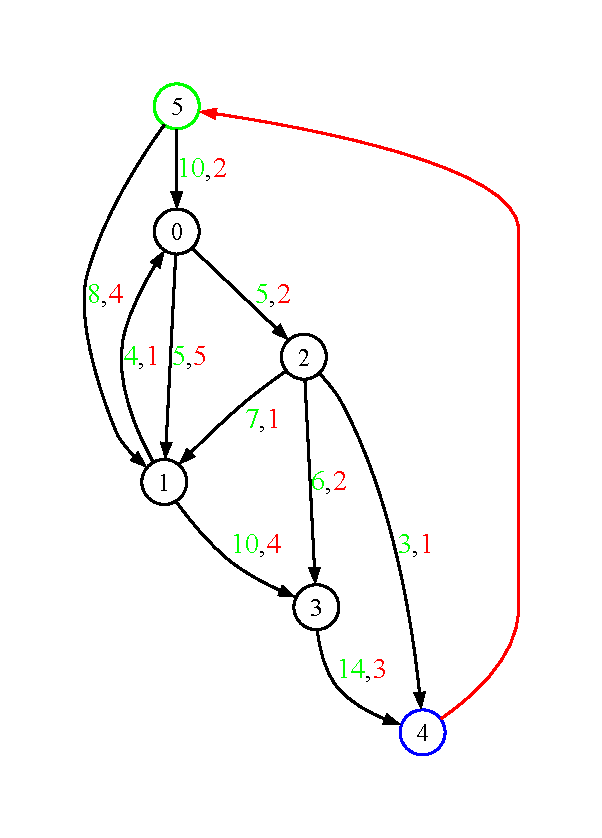
\includegraphics{../output/graph_data/graph.dot.pdf}
  \caption{Le fichier \texttt{output/graph\_data/graph.dot.pdf}}
\end{figure}

\clearpage

\subsubsection{Format du résultat du flot maximum et de la coupe minimum}

Après calcul du flot maximum et de la coupe minimum, le logiciel produit le résultat sous format DOT de Graphviz pour la visualisation.

Pour l'exemple de graphe présenté dans la section \ref{formatentree}, les fichiers \texttt{maxFlowMinCut.dot} et \texttt{maxFlowMinCut.dot.pdf} suivants sont produits :\\
Le fichier \texttt{output/graph\_data/maxFlowMinCut.dot} :

\begin{verbatim}
digraph Gv2MaxFlowMinCut{
    graph [nodesep="0.3", ranksep="0.3",fontsize=12]
    node [shape=circle,fixedsize=true,width=.3,height=.3,fontsize=12]
    edge [arrowsize=0.6]
    label="maximum flow = 15, minimum cut = 15"
    labelloc=t

    5 -> 0 [label = <<font color="blue">7</font>/<font color="green">10</font>>,color=blue,penwidth=1.0]
    5 -> 1 [label = <<font color="blue">8</font>/<font color="green">8</font>>,color=blue,penwidth=1.0]
    0 -> 1 [label = <<font color="blue">2</font>/<font color="green">5</font>>,color=blue,penwidth=1.0]
    0 -> 2 [label = <<font color="blue">5</font>/<font color="green">5</font>>,color=orange,penwidth=2.0]
    1 -> 0 [label = <<font color="blue">0</font>/<font color="green">4</font>>]
    1 -> 3 [label = <<font color="blue">10</font>/<font color="green">10</font>>,color=orange,penwidth=2.0]
    2 -> 1 [label = <<font color="blue">0</font>/<font color="green">7</font>>]
    2 -> 3 [label = <<font color="blue">2</font>/<font color="green">6</font>>,color=blue,penwidth=1.0]
    2 -> 4 [label = <<font color="blue">3</font>/<font color="green">3</font>>,color=blue,penwidth=1.0]
    3 -> 4 [label = <<font color="blue">12</font>/<font color="green">14</font>>,color=blue,penwidth=1.0]
    4 -> 5 [color=red]

    5 [label="5",color=green]
    0 [label="0",style=filled,fillcolor=orange]
    1 [label="1",style=filled,fillcolor=orange]
    2 [label="2",style=filled,fillcolor=orange]
    3 [label="3",style=filled,fillcolor=orange]
    4 [label="4",color=blue]
}

\end{verbatim}

\begin{figure}[hbt]
  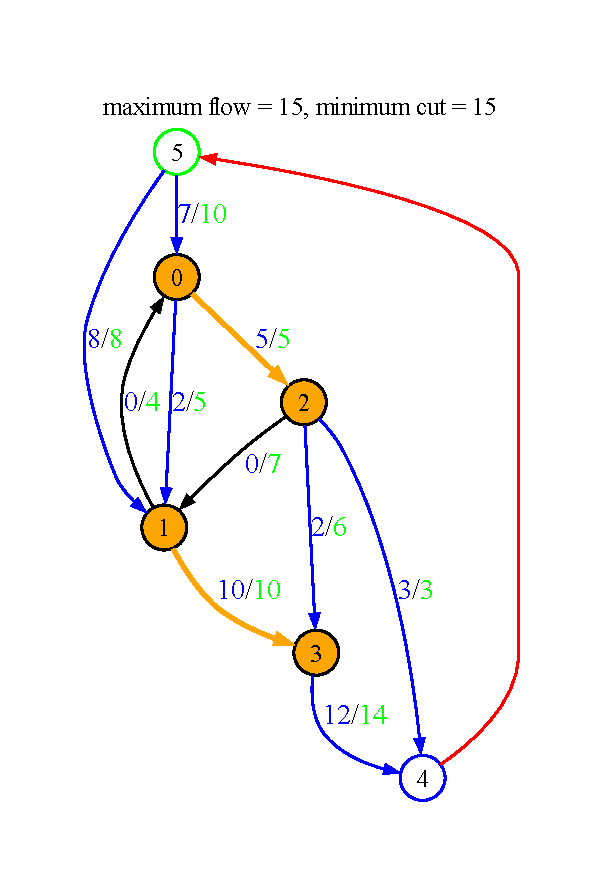
\includegraphics{../output/graph_data/maxFlowMinCut.dot.pdf}
  \caption{Le fichier \texttt{output/graph\_data/maxFlowMinCut.dot.pdf}}
  \label{figgraphdatamaxFlowMinCut}
\end{figure}


\clearpage

Remarque : sur la \autoref{figgraphdatamaxFlowMinCut} ci-dessus, la coupe minimum est représenté par les arcs oranges entre les noeuds oranges. \newline



Les graphes résiduels intermédiaires, utilisés à chaque étape de l'algorithme pour calculer le flot maximum et de la coupe minimum, sont également générés sous format DOT. 

Pour l'exemple de graphe présenté dans la section \ref{formatentree}, les fichiers suivants sont produits :

\begin{verbatim}
output/graph_data/residualGraphs/maxFlowMinCut-residual-0.dot
output/graph_data/residualGraphs/maxFlowMinCut-residual-0.dot.pdf
output/graph_data/residualGraphs/maxFlowMinCut-residual-1.dot
output/graph_data/residualGraphs/maxFlowMinCut-residual-1.dot.pdf
output/graph_data/residualGraphs/maxFlowMinCut-residual-2.dot
output/graph_data/residualGraphs/maxFlowMinCut-residual-2.dot.pdf
output/graph_data/residualGraphs/maxFlowMinCut-residual-3.dot
output/graph_data/residualGraphs/maxFlowMinCut-residual-3.dot.pdf
output/graph_data/residualGraphs/maxFlowMinCut-residual-4.dot
output/graph_data/residualGraphs/maxFlowMinCut-residual-4.dot.pdf
\end{verbatim}

\clearpage

\subsubsection{Format du résultat du flot au coût minimum}

Après calcul du flot au coût minimum, le logiciel produit le résultat sous format DOT de Graphviz pour la visualisation.

Comme il existe deux variantes de résolution de l'algorithme, les résultats de ces deux variantes seront produits. 

La variante basée sur la recherche de plus courts chemins par l'algorithme de Bellman-Ford produit les fichiers \texttt{minimumCostFlowWithPathAlgorithm.dot} et \texttt{minimumCostFlowWithPathAlgorithm.dot.pdf}.

La variante basée sur l'algorithme de Dijkstra avec normalisation des coûts par potentiels produit les fichiers \texttt{minimumCostFlowWithDijkstraAndCostNormalization.dot} et\\ \texttt{minimumCostFlowWithDijkstraAndCostNormalization.dot.pdf}.

Pour l'exemple de graphe présenté dans la section \ref{formatentree}, les fichiers suivants sont ainsi produits :\\
Le fichier \texttt{output/graph\_data/minimumCostFlowWithPathAlgorithm.dot} :

\begin{verbatim}
digraph Gv2MinimumCostFlow{
    graph [nodesep="0.3", ranksep="0.3",fontsize=12]
    node [shape=circle,fixedsize=true,width=.3,height=.3,fontsize=12]
    edge [arrowsize=0.6]
    label="flow = 15, minimum cost = 149"
    labelloc=t

    5 -> 0 [label = <<font color="blue">7</font>/<font color="green">10</font>,<font color="red">2</font>>,color=blue,penwidth=1.0]
    5 -> 1 [label = <<font color="blue">8</font>/<font color="green">8</font>,<font color="red">4</font>>,color=blue,penwidth=1.0]
    0 -> 1 [label = <<font color="blue">2</font>/<font color="green">5</font>,<font color="red">5</font>>,color=blue,penwidth=1.0]
    0 -> 2 [label = <<font color="blue">5</font>/<font color="green">5</font>,<font color="red">2</font>>,color=blue,penwidth=1.0]
    1 -> 0 [label = <<font color="blue">0</font>/<font color="green">4</font>,<font color="red">1</font>>]
    1 -> 3 [label = <<font color="blue">10</font>/<font color="green">10</font>,<font color="red">4</font>>,color=blue,penwidth=1.0]
    2 -> 1 [label = <<font color="blue">0</font>/<font color="green">7</font>,<font color="red">1</font>>]
    2 -> 3 [label = <<font color="blue">2</font>/<font color="green">6</font>,<font color="red">2</font>>,color=blue,penwidth=1.0]
    2 -> 4 [label = <<font color="blue">3</font>/<font color="green">3</font>,<font color="red">1</font>>,color=blue,penwidth=1.0]
    3 -> 4 [label = <<font color="blue">12</font>/<font color="green">14</font>,<font color="red">3</font>>,color=blue,penwidth=1.0]
    4 -> 5 [color=red]

    5 [label="5",color=green]
    0 [label="0"]
    1 [label="1"]
    2 [label="2"]
    3 [label="3"]
    4 [label="4",color=blue]
}

\end{verbatim}

\begin{figure}[hbt]
  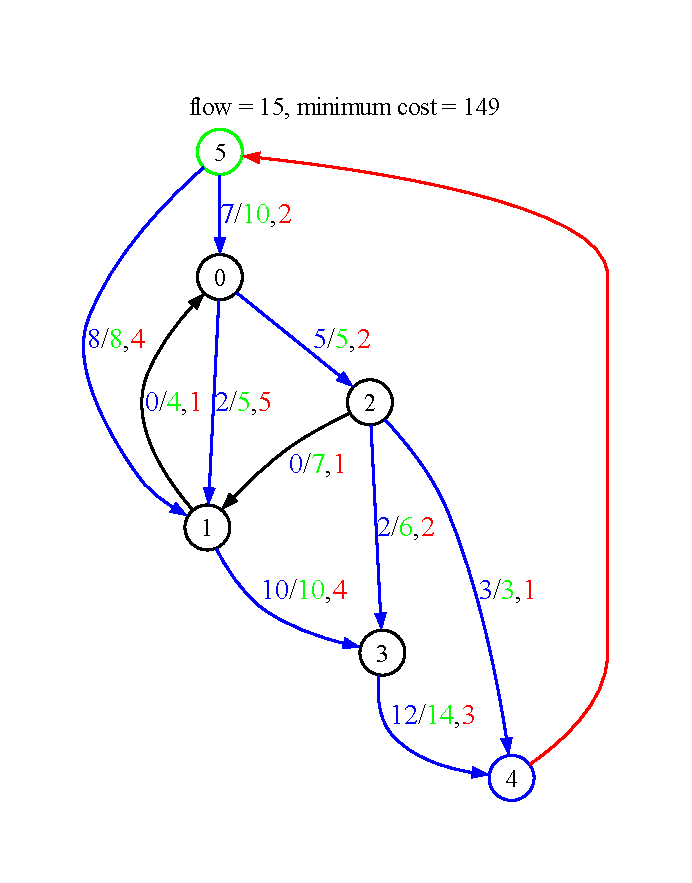
\includegraphics{../output/graph_data/minimumCostFlowWithPathAlgorithm.dot.pdf}
  \caption{Le fichier \texttt{output/graph\_data/minimumCostFlowWithPathAlgorithm.dot.pdf}}
\end{figure}

\clearpage

Le fichier \texttt{output/graph\_data/minimumCostFlowWithDijkstraAndCostNormalization.dot} :

\begin{verbatim}
digraph Gv2MinimumCostFlow{
    graph [nodesep="0.3", ranksep="0.3",fontsize=12]
    node [shape=circle,fixedsize=true,width=.3,height=.3,fontsize=12]
    edge [arrowsize=0.6]
    label="flow = 15, minimum cost = 149"
    labelloc=t

    5 -> 0 [label = <<font color="blue">7</font>/<font color="green">10</font>,<font color="red">2</font>>,color=blue,penwidth=1.0]
    5 -> 1 [label = <<font color="blue">8</font>/<font color="green">8</font>,<font color="red">4</font>>,color=blue,penwidth=1.0]
    0 -> 1 [label = <<font color="blue">2</font>/<font color="green">5</font>,<font color="red">5</font>>,color=blue,penwidth=1.0]
    0 -> 2 [label = <<font color="blue">5</font>/<font color="green">5</font>,<font color="red">2</font>>,color=blue,penwidth=1.0]
    1 -> 0 [label = <<font color="blue">0</font>/<font color="green">4</font>,<font color="red">1</font>>]
    1 -> 3 [label = <<font color="blue">10</font>/<font color="green">10</font>,<font color="red">4</font>>,color=blue,penwidth=1.0]
    2 -> 1 [label = <<font color="blue">0</font>/<font color="green">7</font>,<font color="red">1</font>>]
    2 -> 3 [label = <<font color="blue">2</font>/<font color="green">6</font>,<font color="red">2</font>>,color=blue,penwidth=1.0]
    2 -> 4 [label = <<font color="blue">3</font>/<font color="green">3</font>,<font color="red">1</font>>,color=blue,penwidth=1.0]
    3 -> 4 [label = <<font color="blue">12</font>/<font color="green">14</font>,<font color="red">3</font>>,color=blue,penwidth=1.0]
    4 -> 5 [color=red]

    5 [label="5",color=green]
    0 [label="0"]
    1 [label="1"]
    2 [label="2"]
    3 [label="3"]
    4 [label="4",color=blue]
}

\end{verbatim}

\begin{figure}[hbt]
  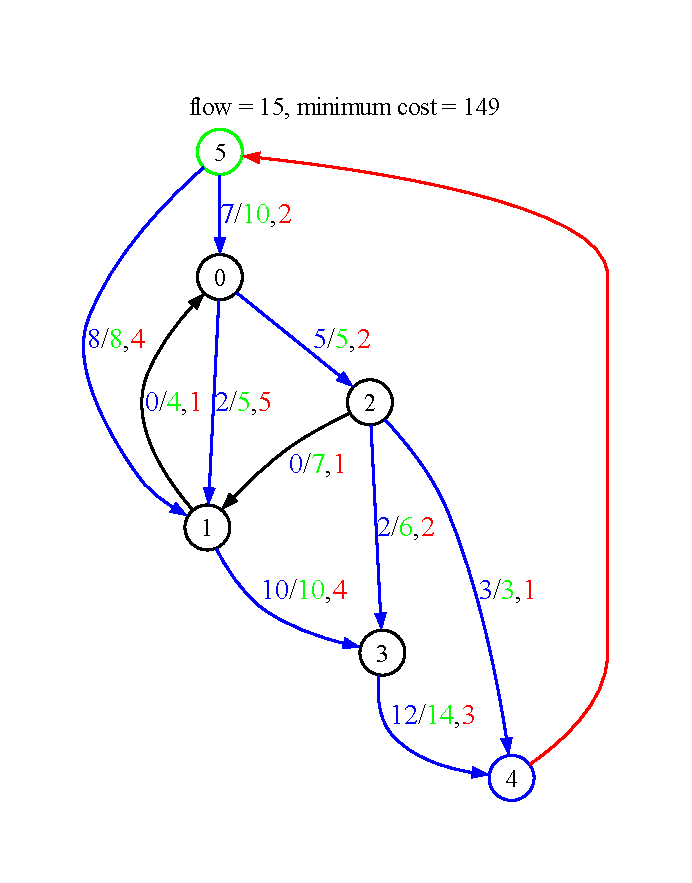
\includegraphics{../output/graph_data/minimumCostFlowWithDijkstraAndCostNormalization.dot.pdf}
  \caption{Le fichier \texttt{output/graph\_data/minimumCostFlowWithDijkstraAndCostNormalization.dot.pdf}}
\end{figure}

\clearpage

Les graphes résiduels intermédiaires, utilisés à chaque étape de l'algorithme pour calculer le flot maximum et de la coupe minimum, sont également générés sous format DOT. 

Pour l'exemple de graphe présenté dans la section \ref{formatentree}, les fichiers suivants sont produits :

\begin{verbatim}
output/graph_data/residualGraphs/minimumCostFlowDijkstraAndCostNormalization-residual-0.dot
output/graph_data/residualGraphs/minimumCostFlowDijkstraAndCostNormalization-residual-0.dot.pdf
output/graph_data/residualGraphs/minimumCostFlowDijkstraAndCostNormalization-residual-1.dot
output/graph_data/residualGraphs/minimumCostFlowDijkstraAndCostNormalization-residual-1.dot.pdf
output/graph_data/residualGraphs/minimumCostFlowDijkstraAndCostNormalization-residual-2.dot
output/graph_data/residualGraphs/minimumCostFlowDijkstraAndCostNormalization-residual-2.dot.pdf
output/graph_data/residualGraphs/minimumCostFlowDijkstraAndCostNormalization-residual-3.dot
output/graph_data/residualGraphs/minimumCostFlowDijkstraAndCostNormalization-residual-3.dot.pdf
output/graph_data/residualGraphs/minimumCostFlowDijkstraAndCostNormalization-residual-4.dot
output/graph_data/residualGraphs/minimumCostFlowDijkstraAndCostNormalization-residual-4.dot.pdf
output/graph_data/residualGraphs/minimumCostFlowPathAlgorithm-residual-0.dot
output/graph_data/residualGraphs/minimumCostFlowPathAlgorithm-residual-0.dot.pdf
output/graph_data/residualGraphs/minimumCostFlowPathAlgorithm-residual-1.dot
output/graph_data/residualGraphs/minimumCostFlowPathAlgorithm-residual-1.dot.pdf
output/graph_data/residualGraphs/minimumCostFlowPathAlgorithm-residual-2.dot
output/graph_data/residualGraphs/minimumCostFlowPathAlgorithm-residual-2.dot.pdf
output/graph_data/residualGraphs/minimumCostFlowPathAlgorithm-residual-3.dot
output/graph_data/residualGraphs/minimumCostFlowPathAlgorithm-residual-3.dot.pdf
output/graph_data/residualGraphs/minimumCostFlowPathAlgorithm-residual-4.dot
output/graph_data/residualGraphs/minimumCostFlowPathAlgorithm-residual-4.dot.pdf
\end{verbatim}

\clearpage

\section{Résultats des exercices}

Pour les exercices donnés dans le document \texttt{DearStudents.docx}, notre programme produit les résultats suivants.

\subsection{Exercice 1 : Calcul du flot maximum}

\subsubsection{Énoncé}

Le premier exercice consiste à calculer le flot maximum dans un réseau de flot orienté. Le réseau est défini par neuf arcs avec leurs capacités respectives.

\subsubsection{Paramètres}

Les noeuds source et puits sont $0$ et $4$ respectivement. Les neuf arcs du réseau sont définis par :

\begin{itemize}
    \item Noeuds source : $[0, 0, 0, 1, 1, 2, 2, 3, 3]$
    \item Noeuds destination : $[1, 2, 3, 2, 4, 3, 4, 2, 4]$
    \item Capacités : $[20, 30, 10, 40, 30, 10, 20, 5, 20]$
\end{itemize}

Chaque arc est défini par ses extrémités source et destination, ainsi que sa capacité maximale.

\subsubsection{Résultats}

Le graphe initial ainsi que le résultat du calcul du flot maximum et coupe minimum sont présentés ci-dessous.

\begin{figure}[hbt]
  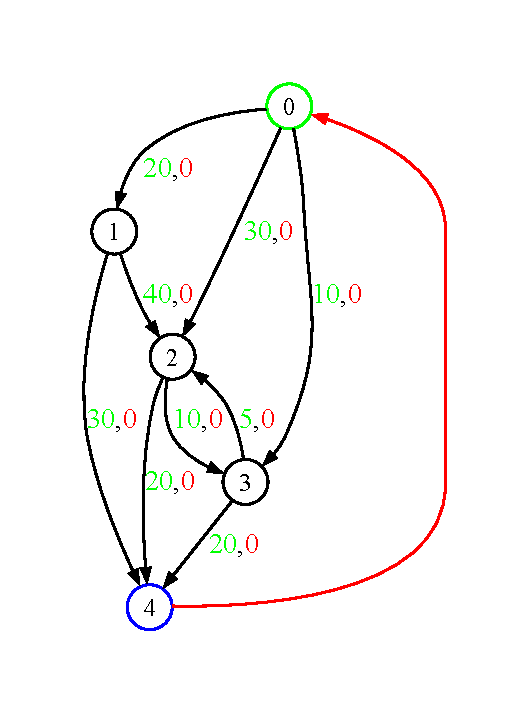
\includegraphics[width=0.8\textwidth]{../output/problem1_graph_data/graph.dot.pdf}
  \caption{Graphe initial pour l'exercice 1,\\ Fichier \texttt{output/problem1\_graph\_data/graph.dot.pdf}}
  \centering
\end{figure}

\begin{figure}[hbt]
  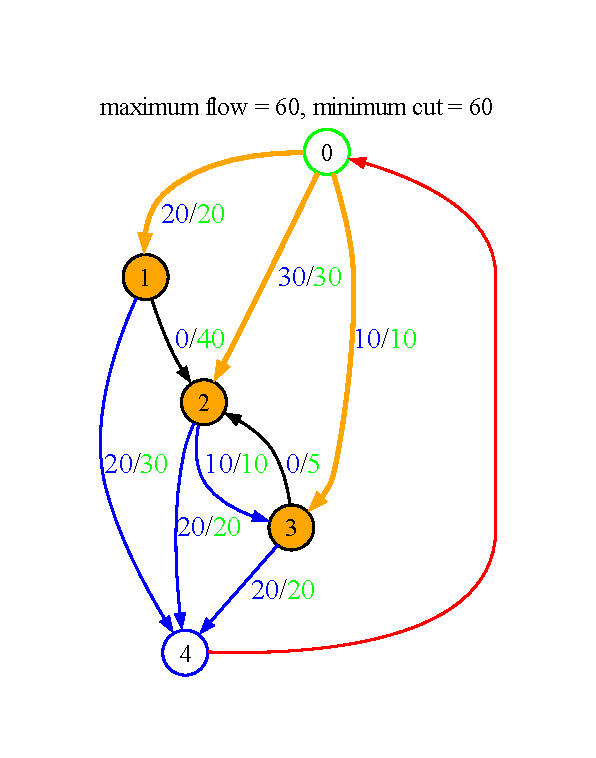
\includegraphics[width=0.8\textwidth]{../output/problem1_graph_data/maxFlowMinCut.dot.pdf}
  \caption{Résultat du flot maximum et de la coupe minimum pour l'exercice 1,\\ Fichier \texttt{output/problem1\_graph\_data/maxFlowMinCut.dot.pdf}}
\end{figure}

\clearpage

\subsection{Exercice 2 : Problème d'affectation à coût minimum}

\subsubsection{Énoncé}

Le deuxième exercice est un problème d'affectation de dix personnes à huit tâches, où chaque affectation a un coût. L'objectif est de trouver une affectation optimale minimisant le coût total. Trois variantes du problème sont considérées selon les contraintes imposées sur la capacité des tâches.

\subsubsection{Paramètres}

Une matrice de coûts de dimension $10 \times 8$ définit le coût d'affectation de chaque personne à chaque tâche. Trois scénarios sont étudiés :

\begin{enumerate}
    \item Sans contrainte de capacité sur les tâches
    \item Avec une capacité maximale de $2$ personnes par tâche
    \item Avec une capacité minimale de $1$ personne par tâche
\end{enumerate}

\subsubsection{Résultats}

Pour chacune des trois variantes, le flot à coût minimum est calculé. Les résultats sont présentés ci-dessous.

\paragraph{Variante 1 : Sans contrainte de capacité}

\begin{figure}[hbt]
  
\includegraphics[width=0.8\textwidth]{../output/problem2-1_graph_data/minimumCostFlowWithPathAlgorithm.dot.pdf}
  \caption{Résultat du flot à coût minimum pour l'exercice 2, variante 1,\\ Fichier \texttt{output/problem2-1\_graph\_data/minimumCostFlowWithPathAlgorithm.dot.pdf}}
\end{figure}

\clearpage

\paragraph{Variante 2 : Avec capacité maximale de 2 personnes par tâche}

\begin{figure}[hbt]
  
\includegraphics[width=0.8\textwidth]{../output/problem2-2_graph_data/minimumCostFlowWithPathAlgorithm.dot.pdf}
  \caption{Résultat du flot à coût minimum pour l'exercice 2, variante 2,\\ Fichier \texttt{output/problem2-2\_graph\_data/minimumCostFlowWithPathAlgorithm.dot.pdf}}
\end{figure}

\paragraph{Variante 3 : Avec capacité maximale de 1 personne par tâche}

\begin{figure}[hbt]
  
\includegraphics[width=0.8\textwidth]{../output/problem2-3_graph_data/minimumCostFlowWithPathAlgorithm.dot.pdf}
  \caption{Résultat du flot à coût minimum pour l'exercice 2, variante 3,\\ Fichier \texttt{output/problem2-3\_graph\_data/minimumCostFlowWithPathAlgorithm.dot.pdf}}
\end{figure}

\clearpage

\subsection{Exercice 3 : Problème de flot à coût minimum avec source et puits}

\subsubsection{Énoncé}

Le troisième exercice porte sur le calcul du flot à coût minimum dans un réseau de flot. Le réseau compte initialement cinq noeuds $(0, 1, 2, 3, 4)$ et neuf arcs. Une source artificielle $s$ et un puits artificiel $t$ sont ajoutés au réseau. Trois variantes du problème sont considérées.

\subsubsection{Paramètres}

Le réseau de flot est initialement défini par :

\begin{itemize}
    \item Noeuds source : $[0, 0, 1, 1, 1, 2, 2, 3, 4]$
    \item Noeuds destination : $[1, 2, 2, 3, 4, 3, 4, 4, 2]$
    \item Capacités : $[15, 8, 20, 4, 10, 15, 4, 20, 5]$
    \item Coûts unitaires : $[4, 4, 2, 2, 6, 1, 3, 2, 3]$
\end{itemize}

Les modifications apportées au réseau sont :
\begin{itemize}
    \item Un arc artificiel de $s$ vers le noeud $0$ avec une capacité de $20$
    \item Un arc de $3$ vers le puits $t$ avec une capacité de $5$
    \item Un arc de $4$ vers le puits $t$ avec une capacité de $15$
\end{itemize}

Les deux variantes étudiées sont :
\begin{enumerate}
    \item Recherche du flot à coût minimum de $s$ vers $t$
    \item Recherche du flot à coût minimum de $0$ vers $4$
\end{enumerate}

\subsubsection{Résultats}

Pour chacune des deux variantes, le flot à coût minimum est calculé. Les résultats sont présentés ci-dessous.

\clearpage

\paragraph{Variante 1 : Flot à coût minimum de $s$ vers $t$}

\begin{figure}[hbt]
  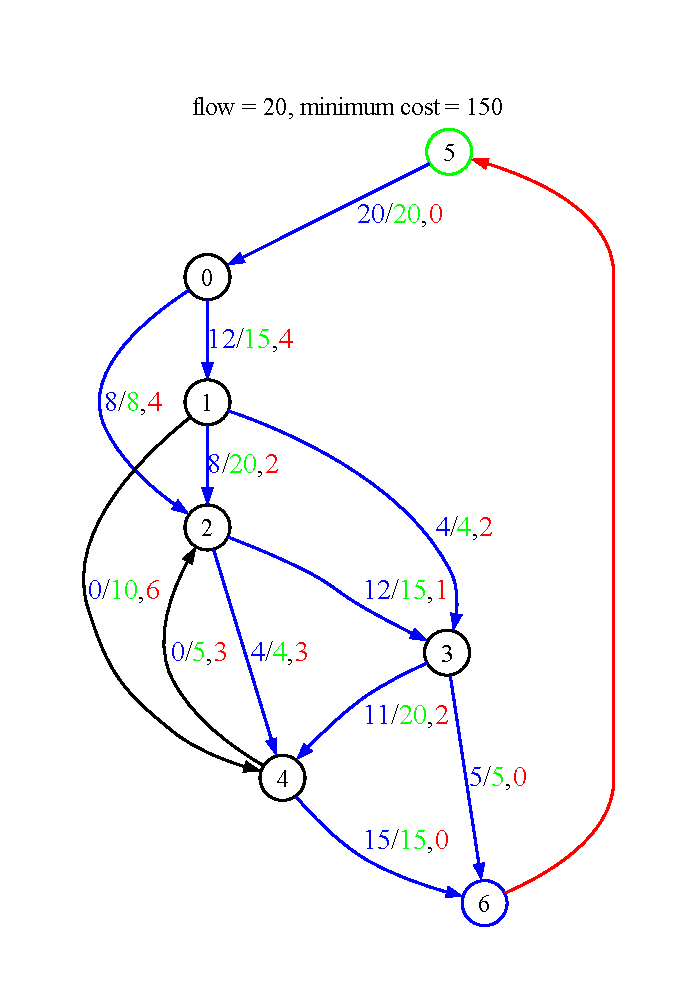
\includegraphics[width=0.7\textwidth]{../output/problem3-1_graph_data/minimumCostFlowWithPathAlgorithm.dot.pdf}
  \caption{Résultat du flot à coût minimum pour l'exercice 3, variante 1,\\ Fichier \texttt{output/problem3-1\_graph\_data/minimumCostFlowWithPathAlgorithm.dot.pdf}}
\end{figure}

\clearpage

\paragraph{Variante 2 : Flot à coût minimum de $0$ vers $4$}

\begin{figure}[hbt]
  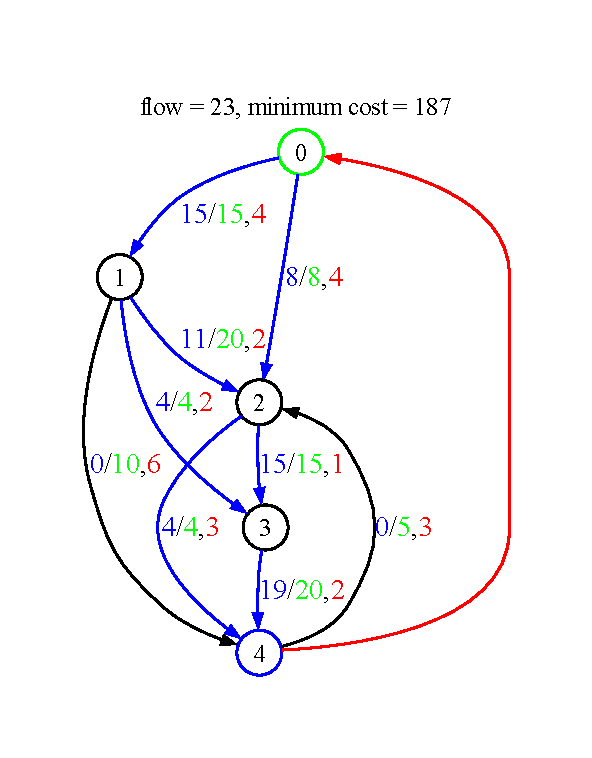
\includegraphics[width=0.7\textwidth]{../output/problem3-2_graph_data/minimumCostFlowWithPathAlgorithm.dot.pdf}
  \caption{Résultat du flot à coût minimum pour l'exercice 3, variante 2,\\ Fichier \texttt{output/problem3-2\_graph\_data/minimumCostFlowWithPathAlgorithm.dot.pdf}}
\end{figure}

\clearpage
 

\section{Conclusion}

Pour conclure, nous avons dans ce projet implémenté plusieurs algorithmes pour manipuler des réseaux de flot.

Premièrement, pour calculer le flot maximum et une coupe minimum, l'algorithme Ford-Fulkerson a été implémenté. Ensuite, pour calculer le flot au coût minimum d'un réseau de flot, un algorithme en deux variantes a été implémenté : une première variante basée sur la recherche de plus courts chemins par l'algorithme de Bellman-Ford, et une seconde variant basée sur l'algorithme de Dijkstra avec normalisation des coûts par potentiels. Finalement, pour détecter si le réseau de flot contient des cycles à coûts négatifs ou non, un l'algorithme reposant sur un variante de Bellman-Ford a été implémenté.

Les exercices du document \texttt{DearStudents.docx} ont également été résolus, et les résultats ont été présentés.


\end{document}
